
\documentclass[aspectratio=169]{beamer}
\usepackage[spanish,es-nodecimaldot]{babel}
\usepackage[utf8]{inputenc}
\usepackage[T1]{fontenc}
\usepackage{lmodern}
\usepackage{booktabs}
\usepackage{array}
\usepackage{ragged2e}
\usepackage{hyperref}
\usepackage{url}
\usetheme{Madrid}
\usecolortheme{default}
\setbeamertemplate{navigation symbols}{}
\setbeamertemplate{footline}

\title{Sistema inteligente de control ESD de bajo costo\\para el laboratorio TestChip Intel Costa Rica}
\subtitle{Estado del arte, marco teórico y definición del problema}
\author{Randy Zamora Rojas}
\institute{Proyecto de graduación -- Ingeniería Electrónica\\Instituto Tecnológico de Costa Rica}
\date{Marzo 2026}

\begin{document}

\begin{frame}
  \titlepage
\end{frame}

\begin{frame}{Motivación}

Una persona puede generar hasta 35,000 V simplemente caminando [2].
Este nivel es suficiente para dañar dispositivos electrónicos sensibles, incluso sin que el daño sea visible.
De hecho, la industria pierde entre un 4\% y 6\% de sus ingresos debido a la electróestática [11].

\begin{figure}
    \centering
    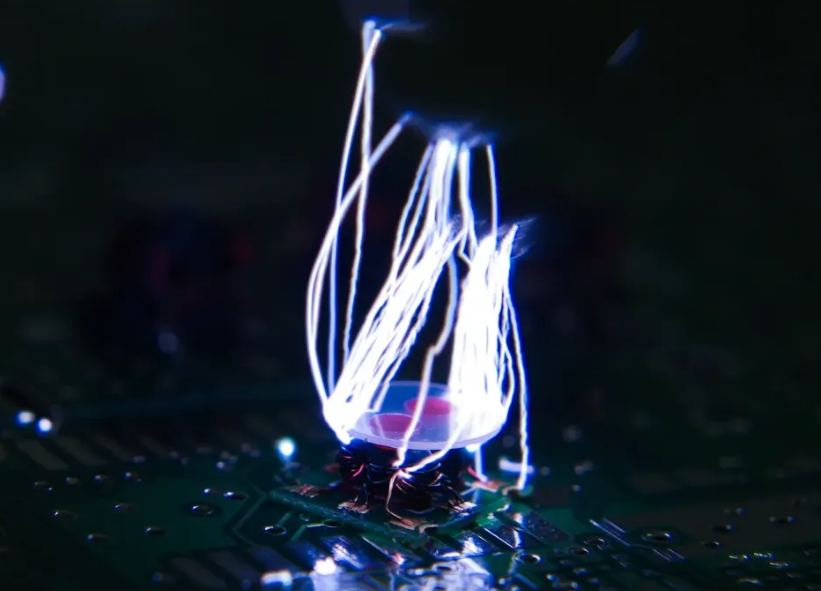
\includegraphics[width=0.4\textwidth]{Figures/F1.png}
\end{figure}

\end{frame}

\begin{frame}{Agenda}
\tableofcontents
\end{frame}

\section{Introducción}
\begin{frame}{Introducción}
\begin{columns}
    \column{0.7\textwidth}
    \begin{figure}[H]
        \centering
        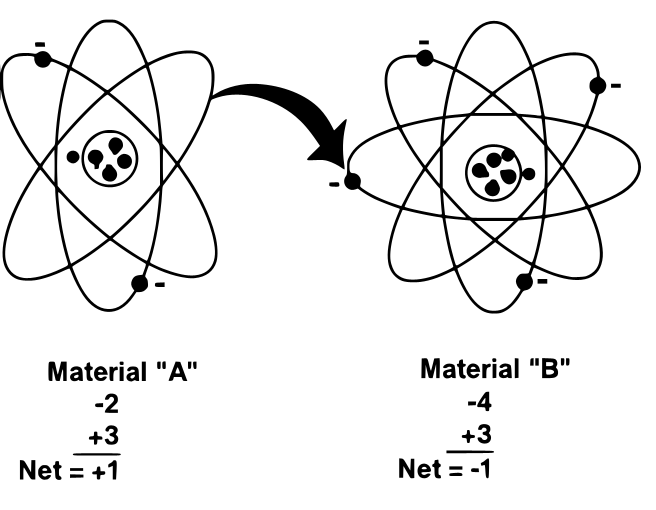
\includegraphics[width=0.9\textwidth]{Figures/F2.png}
    \end{figure}
    \column{0.2\textwidth}
    \begin{equation*}
        \boxed{\text{q} = \text{C} \cdot \text{V}}
    \end{equation*}
\end{columns}
\end{frame}

\begin{frame}{Introducción}
    \centering
    \textbf{Ejemplos de Niveles Típicos de Voltaje de Generación Estática [2]}
    \vspace{0.3cm}
    \small
    \renewcommand{\arraystretch}{1.25}
    \begin{tabular}{|p{5.2cm}|c|c|}
        \hline
        \textbf{Means of Generation} & \textbf{10--25\% RH} & \textbf{65--90\% RH} \\ \hline
        Walking across carpet S           & 35{,}000 V & 1{,}500 V \\ \hline
        Walking across vinyl tile        & 12{,}000 V & 250 V \\ \hline
        Worker at bench                  & 6{,}000 V & 100 V \\ \hline
        Polybag picked up from the bench & 20{,}000 V & 1{,}200 V \\ \hline
        Chair with urethane foam         & 18{,}000 V & 1{,}500 V \\ \hline
    \end{tabular}

    \vspace{0.2cm}
    \raggedleft
    \scriptsize Fuente: [2]
\end{frame}

\begin{frame}{Introducción}
    \begin{figure}
        \centering
        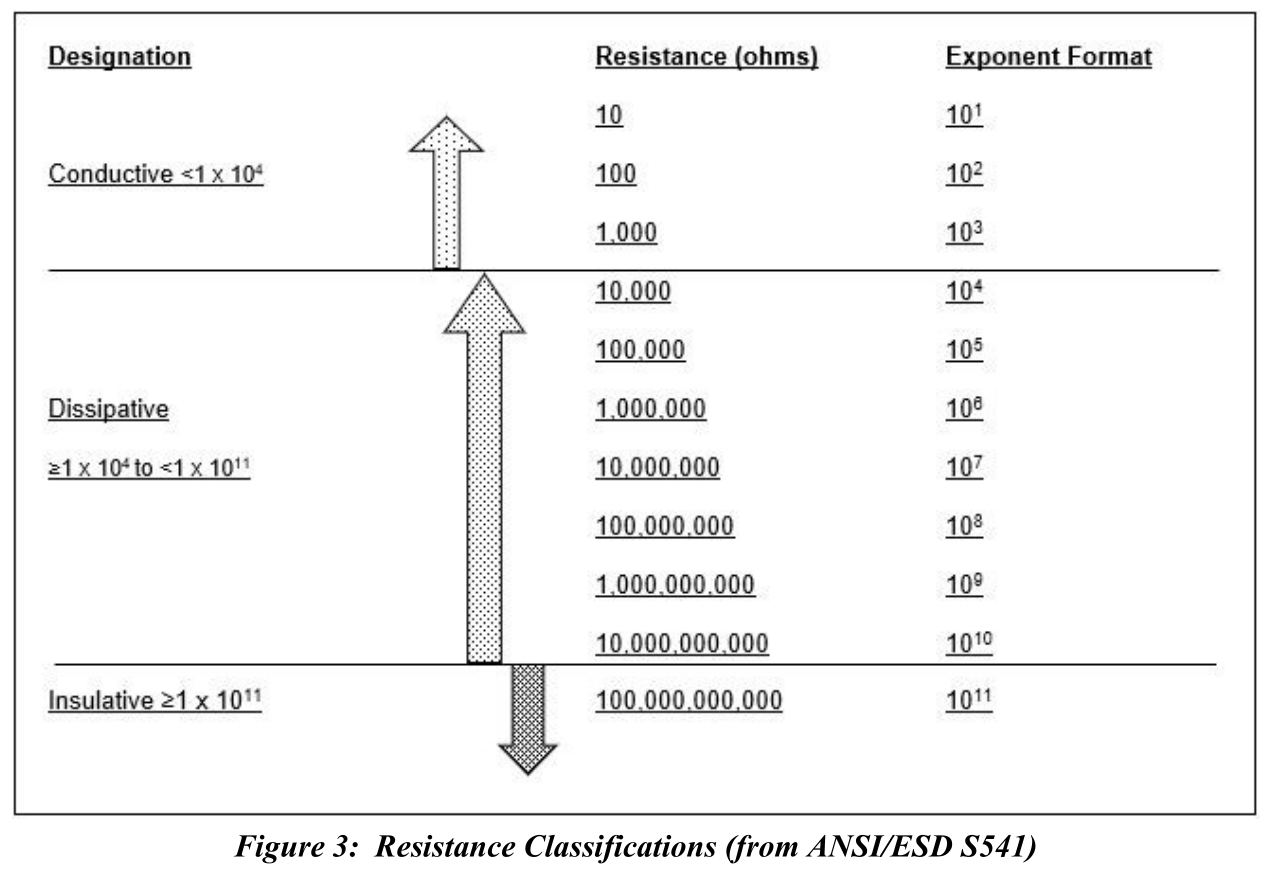
\includegraphics[width=0.6\textwidth]{Figures/F3.png}
    \end{figure}

    \vspace{0.2cm}
    \raggedleft
    \scriptsize Fuente: [2]
\end{frame}

\begin{frame}{Introducción}
    \begin{figure}
        \centering
        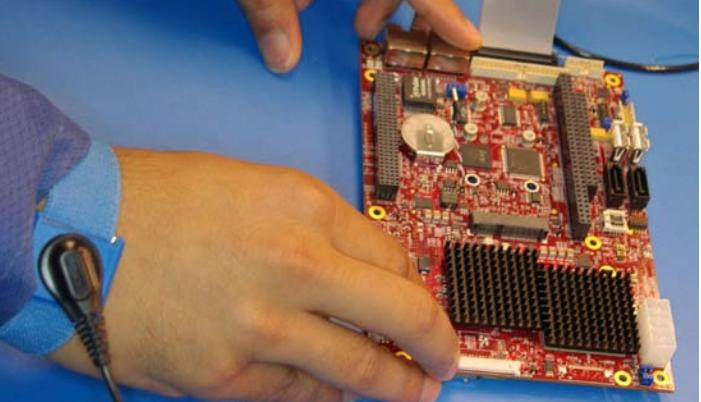
\includegraphics[width=0.6\textwidth]{Figures/F4.jpeg}
    \end{figure}

    \vspace{0.2cm}
    \raggedleft
    \scriptsize Fuente: [11]
\end{frame}

\section{Marco teórico}
\begin{frame}{Marco teórico: generación de carga y daño}
\begin{itemize}
    \item La magnitud de la carga depende del tipo de material, velocidad de separación, área de contacto y humedad relativa [2].
    \item El daño puede ser \textbf{catastrófico} (falla inmediata) o \textbf{latente} (degradación que reduce la vida útil del sistema) [2], [5].
    \item Los estándares de control suelen tomar como base productos con sensibilidad de 100~V HBM y 200~V CDM [1], [9].
\end{itemize}
\end{frame}

\begin{frame}{Marco teórico: puesta a tierra y control de personal}
\begin{itemize}
    \item La puesta a tierra busca mantener conductores, superficies y personal al mismo potencial eléctrico [4], [9], [10].
    \item Las pulseras antiestáticas siguen siendo el método principal para operadores sentados; los sistemas piso/calzado se usan cuando se requiere movilidad [4], [9], [10].
    \item La verificación periódica es obligatoria dentro de un plan de cumplimiento; en pulseras, la práctica común es prueba diaria o monitoreo continuo [4], [8], [9].
    \item La auditoría requiere instrumentos básicos como medidor de campo, medidor de resistencia y probadores de muñequera/calzado [5], [8].
\end{itemize}
\end{frame}

\begin{frame}{Marco teórico: influencia ambiental}
\begin{itemize}
    \item La humedad relativa influye en la acumulación de carga y en la severidad de la descarga; ambientes secos favorecen mayores tensiones y descargas más severas [11], [12], [14].
    \item Sin embargo, la humidificación por sí sola no sustituye un programa ESD completo; debe verse como apoyo al control del riesgo [11], [12], [14].
    \item Literatura reciente también reporta que cambios de temperatura y humedad pueden modificar la robustez ESD de dispositivos de protección integrados [13].
    \item Esto justifica incorporar sensores ambientales como valor agregado del sistema propuesto.
\end{itemize}
\end{frame}

\section{Estado del arte}
\begin{frame}{Estado del arte: estándares y guías}
\begin{itemize}
    \item \textbf{ANSI/ESD S20.20}: documento base para establecer, implementar y mantener un programa de control ESD [1], [19].
    \item \textbf{IEC 61340-5-1}: versión internacional con requisitos administrativos y técnicos para el programa ESD [9].
    \item \textbf{NASA JSC-66552}: referencia de alta confiabilidad para protección de componentes y ensambles electrónicos en ambientes críticos [10].
    \item \textbf{TR53 / TR20.20}: soporte para verificación, auditoría e interpretación práctica del programa [8], [20].
\end{itemize}
\end{frame}

\begin{frame}{Estado del arte: Investigación académica}
\begin{itemize}
    \item También existen enfoques de monitoreo continuo y gestión por tablero para seguimiento del estado de muñequera y cumplimiento [14], [18].
    \item A nivel académico, la literatura se concentra más en monitoreo, protección de dispositivos y efectos ambientales que en estaciones integradas de bajo costo [13], [14].
\end{itemize}
\end{frame}

\begin{frame}{Estado del arte: Probadores de Wrist Straps}

\begin{columns}

\column{0.5\textwidth}
\centering
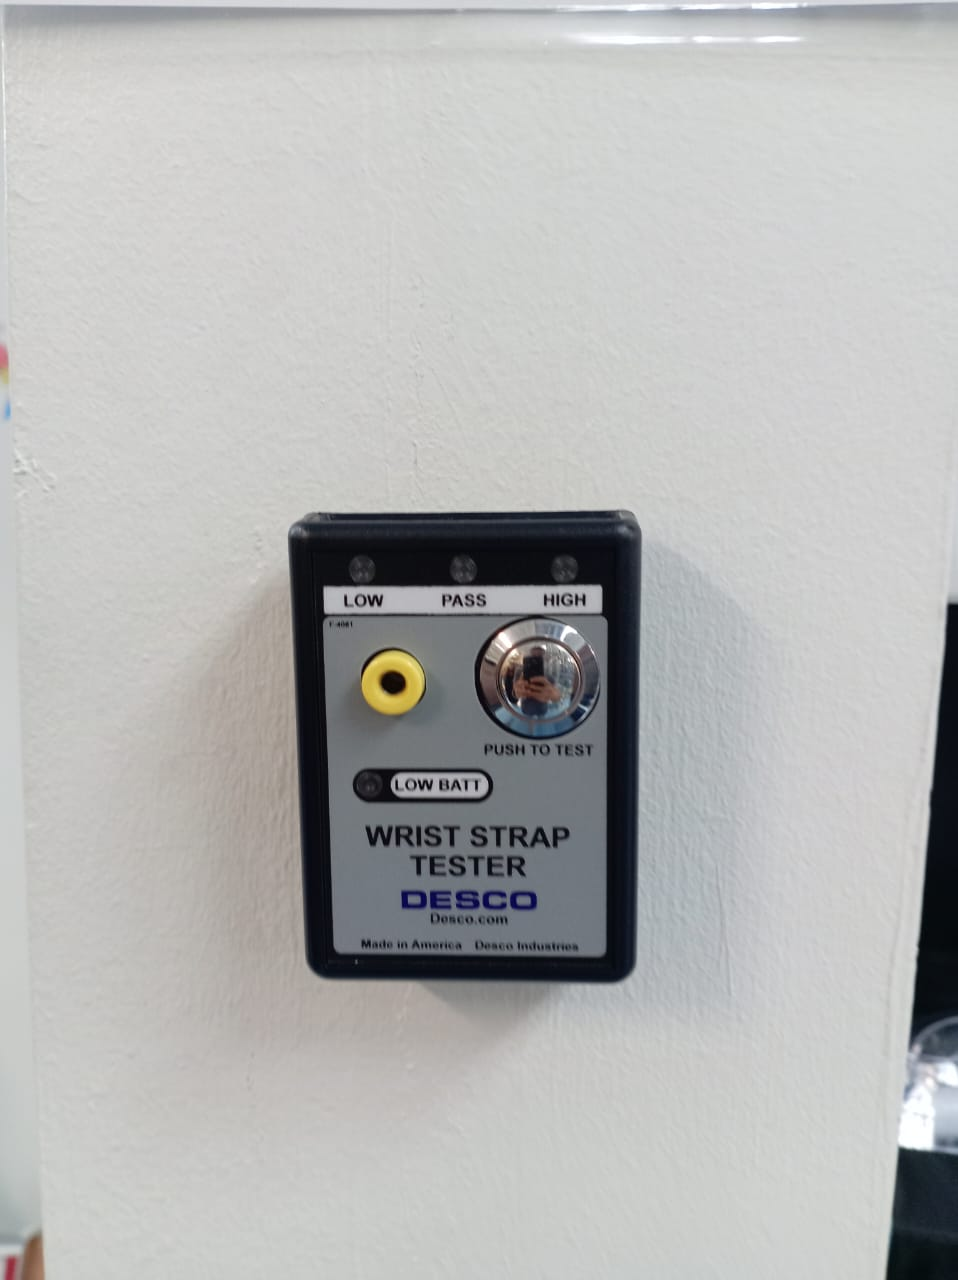
\includegraphics[width=0.6\linewidth]{Figures/F9.jpeg}\\[0.2cm]
{\scriptsize DESCO Wrist Strap Tester, costo: \(\approx\) \$150 [24].}

\column{0.5\textwidth}
\centering
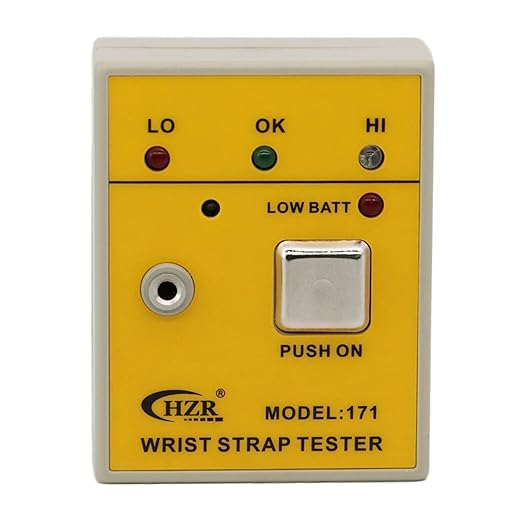
\includegraphics[width=0.8\linewidth]{Figures/F10.jpg}\\[0.2cm]
{\scriptsize HZR 171, costo: \(\approx\) \$30 [20].}

\end{columns}

\end{frame}

\begin{frame}{Estado del arte: Probadores Básicos}

\begin{columns}

\column{0.5\textwidth}
\centering
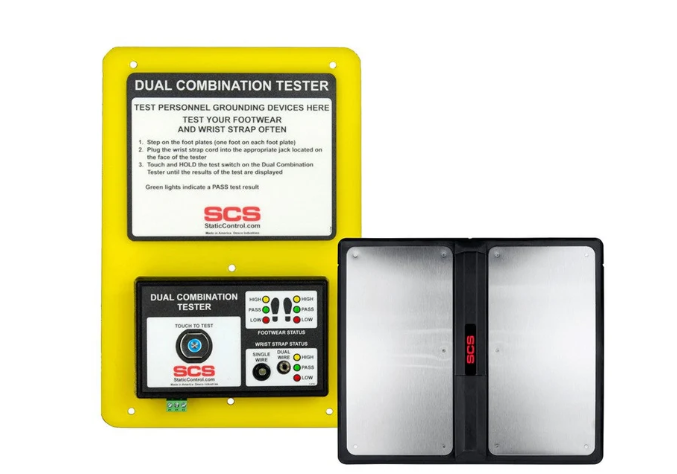
\includegraphics[width=0.6\linewidth]{Figures/F11.png}\\[0.2cm]
{\scriptsize SCS Dual Combination Tester 770758, costo: \(\approx\) \$1073 [25].}

\column{0.5\textwidth}
\centering
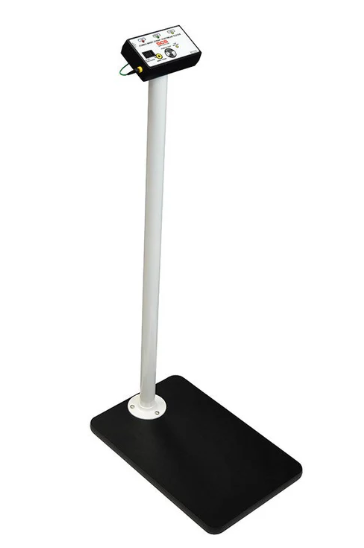
\includegraphics[width=0.5\linewidth]{Figures/F12.png}\\[0.2cm]
{\scriptsize SCS 770031: \(\approx\) \$495 [27].}

\end{columns}

\end{frame}

\begin{frame}{Estado del arte: Estaciones Básicas}

\begin{columns}

\column{0.5\textwidth}
\centering
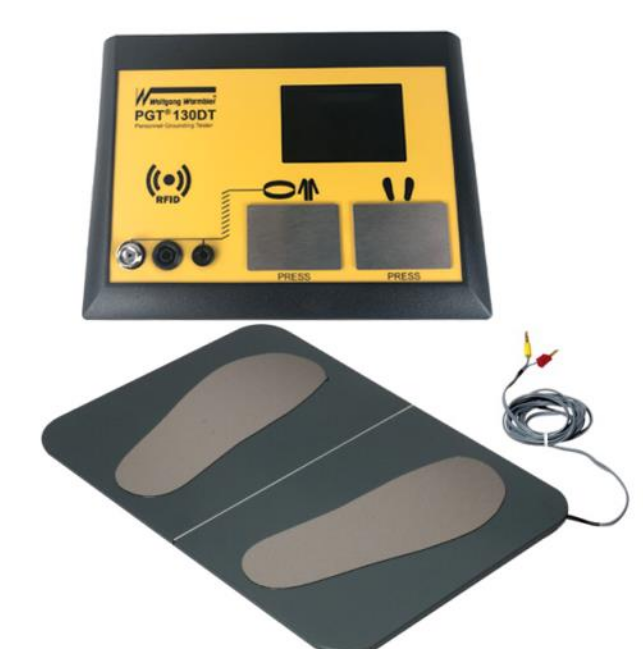
\includegraphics[width=0.6\linewidth]{Figures/F5.png}\\[0.2cm]
{\scriptsize PGT130DT, costo: \(\approx\) \$7676 [23].}

\column{0.5\textwidth}
\centering
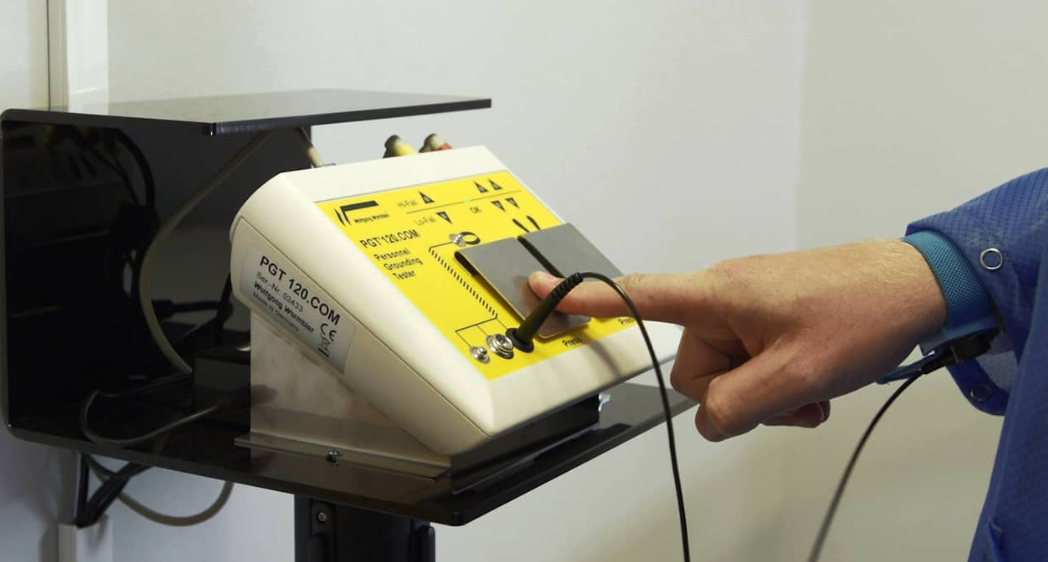
\includegraphics[width=0.8\linewidth]{Figures/F6.png}\\[0.2cm]
{\scriptsize PGT120, costo: \(\approx\) \$2137 [20].}

\end{columns}

\end{frame}

\begin{frame}{Estado del arte: Estaciones Integrales}

\begin{columns}

\column{0.5\textwidth}
\centering
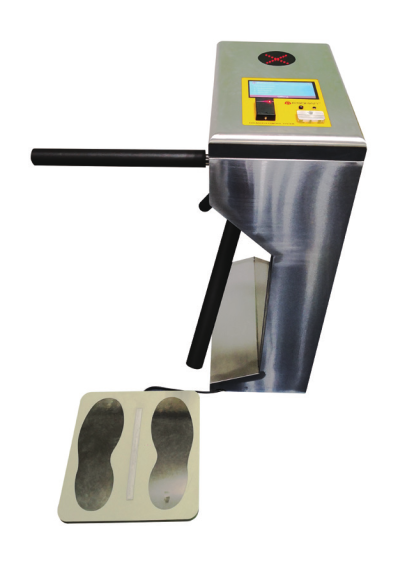
\includegraphics[width=0.6\linewidth]{Figures/F7.png}\\[0.2cm]
{\scriptsize ESDMAN ESD System, costo: \(\approx\) \$2500 [27].}

\column{0.5\textwidth}
\centering
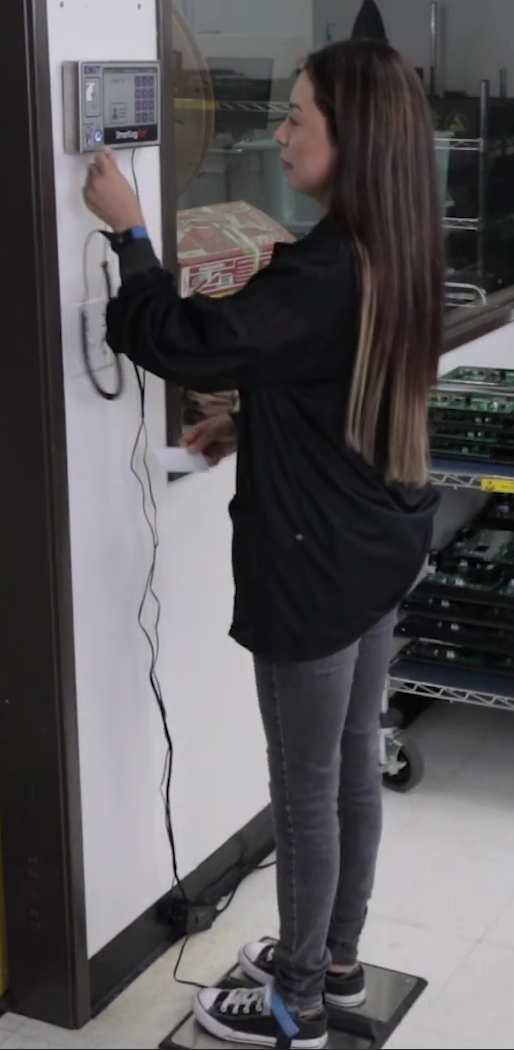
\includegraphics[width=0.4\linewidth]{Figures/F8.png}\\[0.2cm]
{\scriptsize SmartLog Pro 2, costo: \(\approx\) \$5000 [15] [21].}

\end{columns}

\end{frame}

\section{Definición del problema}
\begin{frame}{Definición del problema}
    En el laboratorio TestChip de Intel Costa Rica, 
    se requiere una solución que permita verificar el 
    cumplimiento ESD de forma eficiente, automatizada y de 
    bajo costo, lo cual no es completamente cubierto por las 
    soluciones actuales.
\end{frame}

\begin{frame}{Propuesta preliminar del proyecto}
\begin{figure}
    \centering
    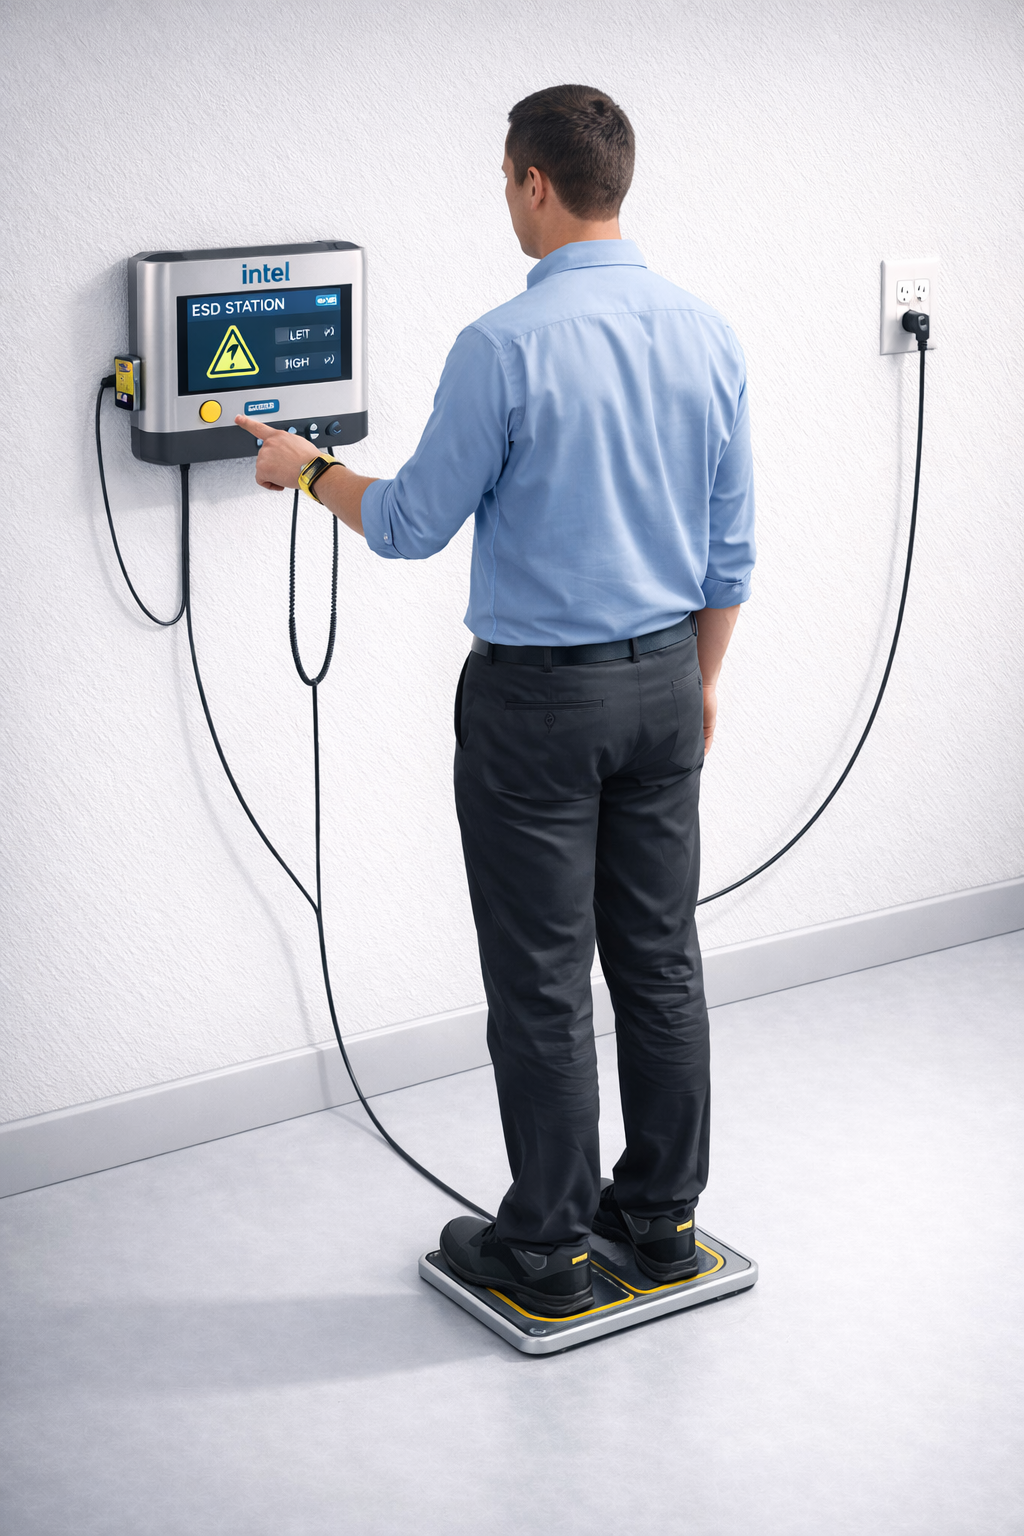
\includegraphics[width=0.31\textwidth]{Figures/F13.png}
\end{figure}
\end{frame}

\section{Conclusiones}
\begin{frame}{Conclusiones}
\begin{itemize}
    \item El estado del arte muestra estándares robustos y productos comerciales útiles, pero deja espacio para una propuesta más accesible y personalizada [10], [14], [15], [18].
    \item La propuesta de una estación ESD inteligente de bajo costo es técnicamente justificable y académicamente relevante.
\end{itemize}
\end{frame}

\appendix
\begin{frame}[fragile]{Referencias [1]--[7]}
\tiny
\begin{enumerate}
\item B. Kelechava, ``ANSI/ESD S20.20-2021: Protection of Electrical and Electronic Parts,'' \emph{ANSI Blog}, Mar. 9, 2022. [En línea]. Disponible en: \url{https://blog.ansi.org/ansi/ansi-esd-s20-20-2021-protection-electronic-parts/}. [Accedido: 23-mar-2026].
\item EOS/ESD Association, ``Fundamentals of Electrostatic Discharge, Part One---An Introduction to ESD,'' 2020. [En línea]. Disponible en: \url{https://www.esda.org/esd-overview/esd-fundamentals/part-1-an-introduction-to-esd/}. [Accedido: 23-mar-2026].
\item EOS/ESD Association, ``Fundamentals of Electrostatic Discharge, Part Two---Principles of ESD Control,'' 2020. [En línea]. Disponible en: \url{https://www.esda.org/esd-overview/esd-fundamentals/part-2-principles-of-esd-control/}. [Accedido: 23-mar-2026].
\item EOS/ESD Association, ``Fundamentals of Electrostatic Discharge, Part Three---Basic ESD Control Procedures and Materials,'' 2020. [En línea]. Disponible en: \url{https://www.esda.org/esd-overview/esd-fundamentals/part-3-basic-esd-control-procedures-and-materials/}. [Accedido: 23-mar-2026].
\item EOS/ESD Association, ``Fundamentals of Electrostatic Discharge, Part Four---Training and Compliance Verification Auditing,'' 2020. [En línea]. Disponible en: \url{https://www.esda.org/esd-overview/esd-fundamentals/part-4-training-and-auditing/}. [Accedido: 23-mar-2026].
\item EOS/ESD Association, ``Fundamentals of Electrostatic Discharge, Part Five---Device Sensitivity and Testing,'' 2024. [En línea]. Disponible en: \url{https://www.esda.org/esd-overview/esd-fundamentals/part-5-device-sensitivity-and-testing/}. [Accedido: 23-mar-2026].
\item EOS/ESD Association, ``Fundamentals of Electrostatic Discharge, Part Six---ESD Standards,'' 2025. [En línea]. Disponible en: \url{https://www.esda.org/esd-overview/esd-fundamentals/part-6-esd-standards/}. [Accedido: 23-mar-2026].
\end{enumerate}
\end{frame}

\begin{frame}[fragile]{Referencias [8]--[14]}
\tiny
\begin{enumerate}
\setcounter{enumi}{7}
\item F. Tenzer y G. Felder, ``ESD Control Program Periodic Verification,'' \emph{Conformity}, mar. 2004. [En línea]. Disponible en: \url{https://desco.descoindustries.com/Articles/ESDControlProgramPeriodic.pdf}. [Accedido: 23-mar-2026].
\item IEC, ``IEC 61340-5-1: Electrostatics---Part 5-1: Protection of electronic devices from electrostatic phenomena---General requirements,'' 2016. [En línea]. Disponible en: \url{https://www.vde-verlag.de/iec-normen/preview-pdf/info_iec61340-5-1%7Bed2.0.RLV%7Den.pdf}. [Accedido: 23-mar-2026].
\item NASA Johnson Space Center, ``JSC-66552: Electrostatic Discharge Control Requirements for the Protection of Electronic Components and Assemblies,'' 2013. [En línea]. Disponible en: \url{https://standards.nasa.gov/sites/default/files/standards/JSC/Baseline/0/JSC-66552BASELINE.pdf}. [Accedido: 23-mar-2026].
\item F. Wan, M. Hillstrom, C. Stayer, D. Swenson y D. Pommerenke, ``The Effect of Humidity on Static Electricity Induced Reliability Issues of ICT Equipment in Data Centers---Motivation and Setup of the Study,'' ASHRAE, 2013. [En línea]. Disponible en: \url{https://www.esdemc.com/public/docs/Publications/Dr.%20Pommerenke%20Related/The%20Effect%20of%20Humidity%20on%20Static%20Electricity%20Induced%20Reliability%20Issues%20of%20ICT%20Equipment%20in%20Data%20Centers%20%E2%80%94Motivation%20and%20Setup%20of%20the%20Study.pdf}. [Accedido: 23-mar-2026].
\item R. Williams, ``Adiabatic \& Isothermal Humidification for Electronics Manufacturing: The Science of Humidity Control in Manufacturing,'' en \emph{Proc. SMTA International}, 2023. [En línea]. Disponible en: \url{https://www.circuitinsight.com/uploads/2/adiabatic-isothermal-humidification-electronics-manufacturing-smta.pdf}. [Accedido: 23-mar-2026].
\item C.-C. Lin y C.-Y. Lin, ``ESD Research of SCR Devices under Harsh Environments,'' \emph{Materials}, vol. 16, no. 18, 2023. [En línea]. Disponible en: \url{https://pmc.ncbi.nlm.nih.gov/articles/PMC10532737/}. [Accedido: 23-mar-2026].
\item ``Monitoring and management of electrostatic wristbands using dashboard,'' prepublicación en ResearchGate, 2024. [En línea]. Disponible en: \url{https://www.researchgate.net/publication/386289271_Monitoring_and_management_of_electrostatic_wristbands_using_dashboard/link/694aef769aa6b4649dc3ebab/download}. [Accedido: 23-mar-2026].
\end{enumerate}
\end{frame}

\begin{frame}[fragile]{Referencias [15]--[20]}
\tiny
\begin{enumerate}
\setcounter{enumi}{14}
\item EMIT, ``SmartLog Pro 2, Hardware 50181.'' [En línea]. Disponible en: \url{https://emit.descoindustries.com/DescoEmitCatalog/Access-Control/SmartLog-Pro-2/Hardware/50181/}. [Accedido: 23-mar-2026].
\item SCS, ``Dual Combination Tester 770758.'' [En línea]. Disponible en: \url{https://staticcontrol.descoindustries.com/SCSCatalog/Wrist-Strap-and-Footwear-Testers/Dual-Combination-Tester/770758/}. [Accedido: 23-mar-2026].
\item Transforming Technologies, ``PGT120 Wolfgang Warmbier Personal Grounding Tester Data Sheet.'' [En línea]. Disponible en: \url{https://transforming-technologies.com/wp-content/uploads/pdf/PGT120-Wolfgang-Warmbier-Personal-Grounding-Tester-Data-Sheet.pdf}. [Accedido: 23-mar-2026].
\item BFN Ionizers, ``PGT130 Wolfgang Warmbier Personal Grounding Tester Data Sheet.'' [En línea]. Disponible en: \url{https://bfnionizers.com/wp-content/uploads/pdf/PGT130.DT-Wolfgang-Warmbier-Personal-Grounding-Tester-Data-Sheet1.pdf}. [Accedido: 23-mar-2026].
\item ESD Association, ``ANSI/ESD S20.20 Standard.'' [En línea]. Disponible en: \url{https://www.esda.org/standards/ansi-esd-s20-20/}. [Accedido: 23-mar-2026].
\item ESD Association, ``ANSI/ESD TR53.'' [En línea]. Disponible en: \url{https://www.esda.org/standards/ansi-esd-tr53/}. [Accedido: 23-mar-2026].
\end{enumerate}
\end{frame}

\begin{frame}[fragile]{Referencias [21]--[26]}
\tiny
\begin{enumerate}
\setcounter{enumi}{20}
\item “Probador antiestático de correa de muñeca,” Amazon, 2024. [En línea]. Disponible en: https://www.amazon.com/-/es/Probador-antiest%C3%A1tico-correa-mu%C3%B1eca-del/dp/B0DDH1TP3J. [Accedido: 23-mar-2026].
\item “ESD Wrist Strap Tester Demo,” YouTube, 2024. [En línea]. Disponible en: https://www.youtube.com/watch?v=D-P-yRWsCyY. [Accedido: 23-mar-2026].
\item “PGT130.DT Data Logging ESD Tester with RFID,” Transforming Technologies, 2024. [En línea]. Disponible en: https://transforming-technologies.com/product/warmbier-pgt130-dt-data-logging-esd-tester-with-rfid/. [Accedido: 23-mar-2026].
\item “Probador de correa de muñeca antiestática,” Amazon, 2024. [En línea]. Disponible en: https://www.amazon.com/-/es/Probador-de-correa-mu%C3%B1eca/dp/B009O10L1O. [Accedido: 23-mar-2026].
\item “SCS 770758 Dual Combination Tester,” Starboard Technologies, 2024. [En línea]. Disponible en: https://starboardtech.com/products/scs-770758-dual-combination-tester. [Accedido: 23-mar-2026].
\item “ESDMAN ESD System,” ESDMAN, 2024. [En línea]. Disponible en: https://www.esdman.com/product/esdman-esd-system/. [Accedido: 23-mar-2026].
\item Starboard Technologies, 2024. [En línea]. Disponible en: https://starboardtech.com/products/scs-770758-dual-combination-tester. [Accedido: 23-mar-2026].
\end{enumerate}
\end{frame}

\end{document}
